\documentclass[aspectratio=1610,polish]{beamer}

\usepackage[utf8]{inputenc}
\usepackage[T1]{fontenc}
\usepackage{polski}
\usepackage{babel}
\usepackage{array}
\usepackage{booktabs}
\usepackage{tikz}
\usetikzlibrary{positioning}

\mode<beamer>{
	\definecolor{links}{HTML}{2A1B81}
	\hypersetup{
		pdfpagemode=FullScreen,
		colorlinks,
		linkcolor=,
		urlcolor=links
	}
	\usetheme[parttitle=rightfooter]{AGH}
}

\title[Klasyfikacja gatunków muzycznych]{Klasyfikacja gatunków muzycznych na podstawie cech audio}
\subtitle{Porównanie cech obliczanych biblioteką \texttt{librosa} z embeddingiem pretrenowanego modelu}
\author[J. Karczewski]{Jakub Karczewski}
\institute[AGH]{Projekt eksploracji danych}
\date{2026}

\newcommand{\acc}[1]{\textbf{#1}}
\newcommand{\smalltable}{\scriptsize}
\setlength{\tabcolsep}{3pt}
\renewcommand{\arraystretch}{1.12}

\begin{document}

\maketitle

\begin{frame}{Cel badania}
	\begin{block}{Pytanie}
		Czy ręcznie obliczane cechy audio z biblioteki \texttt{librosa} są wystarczające do klasyfikacji gatunku muzycznego, czy lepszą reprezentację daje embedding z modelu pretrained?
	\end{block}

	\begin{itemize}
		\item Problem: wieloklasowa klasyfikacja 8 gatunków muzycznych.
		\item Dane wejściowe: tylko sygnał audio, bez tekstu, wykonawcy ani metadanych opisowych.
		\item Porównanie obejmuje trzy notebooki eksperymentalne oraz modele klasyfikacyjne trenowane na tych samych etykietach.
	\end{itemize}
\end{frame}

\begin{frame}{Zbiór danych: FMA Small}
	\begin{columns}
		\column{0.54\textwidth}
		\begin{itemize}
			\item Free Music Archive, wariant \textbf{FMA Small}.
			\item Około \textbf{8000 utworów}.
			\item Oryginalny podział FMA na zbiór treningowy oraz walidacyjno-testowy.
			\item W eksperymencie z embeddingami: 6400 utworów treningowych, z czego 6 odrzucono przez błędy przetwarzania; 1600 utworów walidacyjno-testowych.
		\end{itemize}

		\column{0.42\textwidth}
		\begin{block}{Gatunki}
			\small
			Electronic, Experimental, Folk, Hip-Hop, Instrumental, International, Pop, Rock
		\end{block}
	\end{columns}
\end{frame}

\begin{frame}{Porównywane reprezentacje audio}
	\scriptsize
	\begin{tabular}{p{0.18\textwidth}p{0.31\textwidth}p{0.13\textwidth}p{0.29\textwidth}}
		\toprule
		Eksperyment & Strategia cech & Liczba cech & Reprezentacja \\
		\midrule
		librosa 70 &
		librosa, zestaw zredukowany &
		70 &
		MFCC, chroma, RMS, centroid, ZCR \\
		librosa 518 &
		librosa, zestaw rozszerzony &
		518 &
		szerszy zestaw deskryptorów i statystyk \\
		Cnn14/PANNs &
		embedding modelu pretrained &
		2048 &
		PANNs/Cnn14 przez \texttt{panns\_inference} \\
		\bottomrule
	\end{tabular}
\end{frame}

\begin{frame}{Pipeline eksperymentalny}
	\centering
	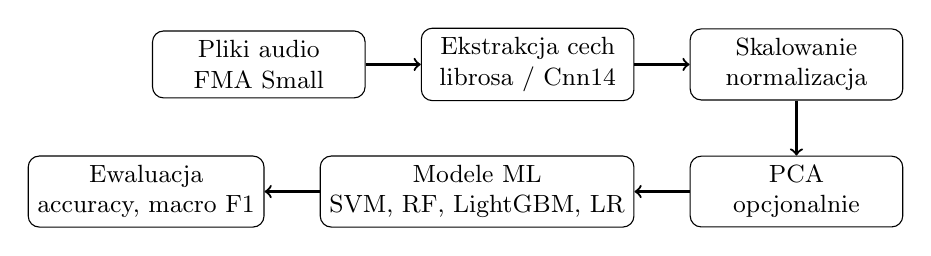
\begin{tikzpicture}[
		node distance=0.7cm,
		box/.style={draw, rounded corners, align=center, minimum width=2.7cm, minimum height=0.85cm, font=\small},
		arrow/.style={->, thick}
	]
		\node[box] (audio) {Pliki audio\\FMA Small};
		\node[box, right=of audio] (features) {Ekstrakcja cech\\librosa / Cnn14};
		\node[box, right=of features] (prep) {Skalowanie\\normalizacja};
		\node[box, below=of prep] (pca) {PCA\\opcjonalnie};
		\node[box, left=of pca] (models) {Modele ML\\SVM, RF, LightGBM, LR};
		\node[box, left=of models] (eval) {Ewaluacja\\accuracy, macro F1};

		\draw[arrow] (audio) -- (features);
		\draw[arrow] (features) -- (prep);
		\draw[arrow] (prep) -- (pca);
		\draw[arrow] (pca) -- (models);
		\draw[arrow] (models) -- (eval);
	\end{tikzpicture}

	\vspace{0.8em}
	\begin{itemize}
		\item Dla cech librosa zastosowano \texttt{StandardScaler}; testowano PCA do 4 komponentów oraz wariant bez PCA.
		\item Dla embeddingów Cnn14 zastosowano normalizację L2; PCA zachowujące 95\% wariancji dało 182 komponenty.
	\end{itemize}
\end{frame}

\begin{frame}{Modele i metryki}
	\begin{columns}
		\column{0.48\textwidth}
		\begin{block}{Modele}
			\begin{itemize}
				\item SVM: kernel liniowy i RBF
				\item Random Forest
				\item LightGBM
				\item Logistic Regression
			\end{itemize}
		\end{block}

		\column{0.48\textwidth}
		\begin{block}{Metryki}
			\begin{itemize}
				\item Accuracy na zbiorze testowym
				\item Macro F1
				\item Raporty precision/recall/F1
				\item Macierze pomyłek
			\end{itemize}
		\end{block}
	\end{columns}
\end{frame}

\begin{frame}{Wyniki: librosa, 70 cech}
	\smalltable
	\begin{tabular}{p{0.30\textwidth}p{0.20\textwidth}ccc}
		\toprule
		Reprezentacja & Model & Train acc. & Test acc. & Macro F1 \\
		\midrule
		PCA, 4 komponenty & SVM liniowy & 0.342 & 0.339 & 0.31 \\
		PCA, 4 komponenty & Random Forest & 0.452 & 0.329 & 0.31 \\
		Bez PCA & Random Forest & 0.598 & 0.438 & 0.42 \\
		Bez PCA & SVM RBF & 0.506 & \acc{0.446} & 0.43 \\
		Bez PCA & LightGBM & 0.738 & 0.444 & \acc{0.44} \\
		Bez PCA & Logistic Regression & 0.506 & 0.394 & 0.39 \\
		\bottomrule
	\end{tabular}

	\vspace{0.6em}
	\begin{itemize}
		\item Najlepszy wynik accuracy: około \textbf{44.6\%}.
		\item PCA do 4 komponentów znacząco pogarsza jakość klasyfikacji.
	\end{itemize}
\end{frame}

\begin{frame}{Wyniki: librosa, 518 cech}
	\smalltable
	\begin{tabular}{p{0.30\textwidth}p{0.20\textwidth}ccc}
		\toprule
		Reprezentacja & Model & Train acc. & Test acc. & Macro F1 \\
		\midrule
		PCA, 4 komponenty & SVM liniowy & 0.340 & 0.317 & 0.27 \\
		PCA, 4 komponenty & Random Forest & 0.436 & 0.324 & 0.31 \\
		Bez PCA & Random Forest & 0.653 & 0.460 & 0.44 \\
		Bez PCA & SVM RBF & 0.441 & 0.411 & 0.39 \\
		Bez PCA & LightGBM & 0.844 & \acc{0.472} & \acc{0.47} \\
		Bez PCA & Logistic Regression & 0.705 & 0.449 & 0.45 \\
		\bottomrule
	\end{tabular}

	\vspace{0.6em}
	\begin{itemize}
		\item Rozszerzenie liczby cech z 70 do 518 poprawia wynik, ale umiarkowanie: z 44.6\% do 47.2\%.
		\item LightGBM osiąga najlepszy wynik, lecz różnica train/test wskazuje na przeuczenie.
	\end{itemize}
\end{frame}

\begin{frame}{Wyniki: embeddingi pretrained}
	\scriptsize
	\begin{tabular}{p{0.29\textwidth}p{0.20\textwidth}ccc}
		\toprule
		Reprezentacja & Model & Train acc. & Test acc. & Macro F1 / wynik \\
		\midrule
		2048-d, L2, bez PCA & LightGBM & -- & 0.610 & 0.610 \\
		PCA, 182 komponenty & LightGBM & 0.817 & 0.599 & 0.595 \\
		PCA, 182 komponenty & Log. Regression & 0.672 & \acc{0.611} & \acc{0.610} \\
		PCA, 182 komponenty & Random Forest & 0.998 & 0.603 & CV macro F1: 0.631 \\
		\bottomrule
	\end{tabular}

	\vspace{0.6em}
	\begin{itemize}
		\item Najlepszy wynik testowy: \textbf{61.1\% accuracy} dla regresji logistycznej.
		\item Prosty model liniowy działa dobrze, ponieważ embedding zawiera bogatszą reprezentację dźwięku.
	\end{itemize}
\end{frame}

\begin{frame}{Porównanie najlepszych konfiguracji}
	\scriptsize
	\begin{tabular}{p{0.34\textwidth}ccc}
		\toprule
		Konfiguracja & Test accuracy & Macro F1 & Różnica \\
		\midrule
		Najlepszy wariant librosa, 70 cech & 0.446 & 0.43 & punkt odniesienia \\
		Najlepszy wariant librosa, 518 cech & 0.472 & 0.47 & najlepsze librosa \\
		Najlepszy wariant embeddingów & \acc{0.611} & \acc{0.610} & +0.139 względem full librosa \\
		\bottomrule
	\end{tabular}

	\vspace{0.7em}
	\centering
	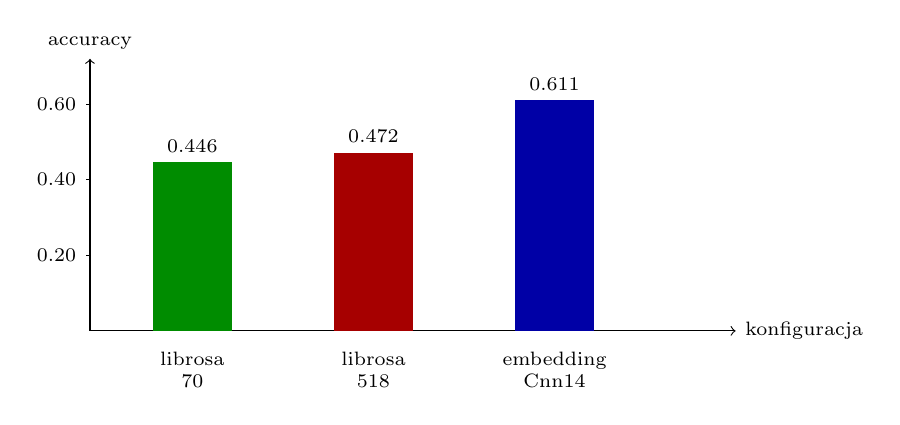
\begin{tikzpicture}[x=1cm,y=4.8cm]
		\draw[->] (0,0) -- (8.2,0) node[right] {\scriptsize konfiguracja};
		\draw[->] (0,0) -- (0,0.72) node[above] {\scriptsize accuracy};
		\foreach \y/\label in {0.2/0.20,0.4/0.40,0.6/0.60}
			\draw (0,\y) -- (-0.05,\y) node[left] {\scriptsize \label};
		\fill[green!55!black] (0.8,0) rectangle (1.8,0.446);
		\fill[red!65!black] (3.1,0) rectangle (4.1,0.472);
		\fill[blue!65!black] (5.4,0) rectangle (6.4,0.611);
		\node[below, align=center, font=\scriptsize] at (1.3,-0.03) {librosa\\70};
		\node[below, align=center, font=\scriptsize] at (3.6,-0.03) {librosa\\518};
		\node[below, align=center, font=\scriptsize] at (5.9,-0.03) {embedding\\Cnn14};
		\node[above, font=\scriptsize] at (1.3,0.446) {0.446};
		\node[above, font=\scriptsize] at (3.6,0.472) {0.472};
		\node[above, font=\scriptsize] at (5.9,0.611) {0.611};
	\end{tikzpicture}
\end{frame}

\begin{frame}{Interpretacja wyników}
	\begin{itemize}
		\item Ręcznie obliczane cechy librosa dają sensowny baseline, ale ich najlepszy wynik pozostaje poniżej 50\% accuracy.
		\item Większy zestaw cech librosa poprawia jakość, ale nie usuwa ograniczenia wynikającego z niskopoziomowego opisu sygnału.
		\item Embedding Cnn14 powstał w wyniku uczenia na dużym zadaniu audio-taggingu, więc przenosi informację o barwie, instrumentacji, rytmie i strukturze czasowo-częstotliwościowej.
		\item Wariant pretrained poprawia accuracy o około \textbf{13.9 punktu procentowego} względem najlepszego wariantu librosa.
	\end{itemize}
\end{frame}

\begin{frame}{Zachowanie na poziomie gatunków}
	\begin{columns}
		\column{0.48\textwidth}
		\begin{block}{Najczęściej prawidłowo przewidywane klasy}
			\begin{itemize}
				\item Rock
				\item Hip-Hop
				\item Electronic
			\end{itemize}
		\end{block}

		\column{0.48\textwidth}
		\begin{alertblock}{Najtrudniejsza do poprawnego przypisania klasa}
			\begin{itemize}
				\item Pop
			\end{itemize}
		\end{alertblock}
	\end{columns}

	\vspace{0.8em}
	Najcześciej mylone klasy: Rock vs Pop, Folk vs International, Electronic vs Experimental oraz Instrumental vs Folk/International. Wynika to z nakładania się stylów.
\end{frame}

\begin{frame}{Wnioski}
	\begin{enumerate}
		\item Cechy librosa są interpretowalne i tanie obliczeniowo, ale mają ograniczoną zdolność separowania gatunków.
		\item PCA do 4 komponentów w eksperymentach librosa usuwa zbyt dużo informacji.
		\item Embeddingi pretrained są wyraźnie skuteczniejsze: najlepsze accuracy rośnie z 47.2\% do 61.1\%.
		\item Najbardziej praktyczny wariant w tych eksperymentach to embedding Cnn14 + PCA 95\% + Logistic Regression.
	\end{enumerate}

	\begin{block}{Wniosek ogólny}
		Dla klasyfikacji gatunków muzycznych transfer learning daje znacznie bogatszą reprezentację niż same ręcznie projektowane deskryptory audio.
	\end{block}
\end{frame}

\begin{frame}{Bibliografia}
	\begin{thebibliography}{9}
		\setbeamertemplate{bibliography item}[article]
		\bibitem{fma} M. Defferrard, K. Benzi, P. Vandergheynst, X. Bresson, \textit{FMA: A Dataset For Music Analysis}, 2017.
		\setbeamertemplate{bibliography item}[online]
		\bibitem{fmarepo} Free Music Archive dataset repository: \url{https://github.com/mdeff/fma}
		\bibitem{librosa} Librosa documentation: \url{https://librosa.org}
		\bibitem{sklearn} Scikit-learn documentation: \url{https://scikit-learn.org}
		\bibitem{lightgbm} LightGBM documentation: \url{https://lightgbm.readthedocs.io}
		\setbeamertemplate{bibliography item}[article]
		\bibitem{panns} Q. Kong et al., \textit{PANNs: Large-Scale Pretrained Audio Neural Networks for Audio Pattern Recognition}.
	\end{thebibliography}
\end{frame}

\end{document}
